\chapter{Fenomeni elettromagnetici}

\section*{Caratteristiche}
\begin{itemize}
    \item \textbf{Grandezze fisiche}
    \begin{figure}[h!]
        \centering
        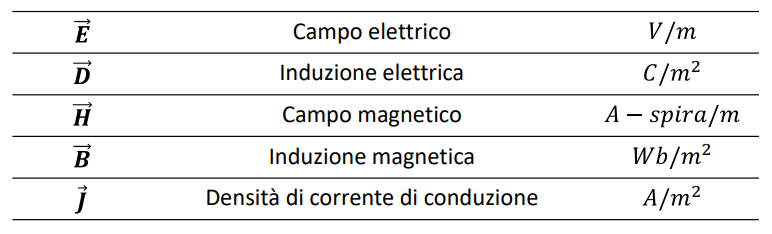
\includegraphics[width=0.7\textwidth]{capitoli/capitolo3/immagini/image1.png}
    \end{figure}
    \begin{itemize}
        \item Vettoriali
        \item Funzione del punto e del tempo
    \end{itemize}

    \item \textbf{Parametri rappresentativi}
    \begin{figure}[h!]
        \centering
        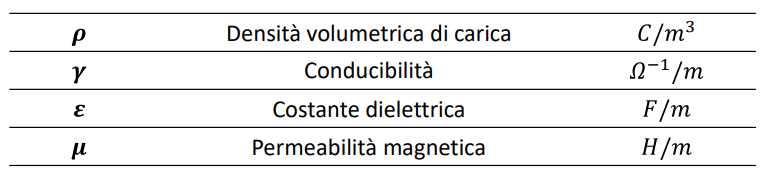
\includegraphics[width=0.7\textwidth]{capitoli/capitolo3/immagini/image2.png}
    \end{figure}

    \vspace{9cm}

    \item \textbf{Equazioni di Maxwell}
    \begin{table}[h]
        \centering
        \renewcommand{\arraystretch}{1.5}
        \begin{tabular}{|l c|}
            \hline
            \textbf{1° Equazione} & \( \nabla \cdot \vec{D} = \rho \) \\
            \hline
            \textbf{2° Equazione} & \( \nabla \cdot \vec{B} = 0 \) \\
            \hline
            \textbf{3° Equazione} & \( \nabla \times \vec{E} = -\frac{\partial \vec{B}}{\partial t} \) \\
            \hline
            \textbf{4° Equazione} & \( \nabla \times \vec{H} = \vec{J} + \frac{\partial \vec{D}}{\partial t} \) \\
            \hline
        \end{tabular}
    \end{table}

    \item \textbf{Relazioni costitutive dei materiali}
    \begin{itemize}
        \item \(\vec{D} = \varepsilon \vec{E} \)
        \item \(\vec{B} = \mu \vec{H} \)
        \item \(\vec{J} = \vec{J_0}+\gamma(\vec{E}-\vec{E_0}) \)
    \end{itemize}
\end{itemize}

\section*{Ipotesi delle costanti concentrate}
\begin{itemize}
    \item Approssimazione del fenomeno elettromagnetico
    \item Dimensioni della struttura trascurabili
    \item Velocit\`a di propagazione \textbf{infinita}
    \item Tempo nullo di trasmissione
    \item Ipotesi valide solo se:
    \begin{itemize}
        \item Tempo di trasmissione \( \ll \) variazioni temporali
        \item Dimensioni spaziali \( \ll \lambda_{min} \)
        \item \( 2 \cdot L_{max} / c \cdot f_{max} \ll 1 \)
    \end{itemize}
\end{itemize}

\section*{Conseguenze delle ipotesi a costanti concentrate}
\begin{itemize}
    \item Velocit\`a di propagazione infinita
    \item Classificazione delle regioni:
    \begin{description}
        \item[\( \varepsilon = 0, \mu = 0 \)] Nessuna energia immagazzinata
        \begin{itemize}
            \item Corrente entrante = corrente uscente
            \item Campo elettrico conservativo
        \end{itemize}
        
        \item[Vuoto ideale]
        \begin{itemize}
            \item Nessuna sollecitazione
            \item \( \sigma = 0 \): non passa corrente
        \end{itemize}

        \vspace{1cm}

        \item[Conduttore ideale]
        \begin{itemize}
            \item \( \sigma \rightarrow \infty \)
            \item Regione equipotenziale
        \end{itemize}

        \item[Resistore]
        \begin{itemize}
            \item \( \sigma \) finita
            \item Dissipazione di potenza
        \end{itemize}

        \item[Generatore indip. di corrente]
        \begin{itemize}
            \item \( \sigma = 0 \)
            \item Trasformazione di energia
        \end{itemize}

        \item[Generatore indip. di tensione]
        \begin{itemize}
            \item \( \sigma \rightarrow \infty \)
            \item Trasformazione di energia
        \end{itemize}

        \item[\( \varepsilon \neq 0, \mu = 0 \): Condensatore]
        \begin{itemize}
            \item Energia elettrica presente
            \item Potenziale definito univocamente
        \end{itemize}

        \item[\( \varepsilon = 0, \mu \neq 0 \): Induttore]
        \begin{itemize}
            \item Energia magnetica presente
            \item Corrente entrante = corrente uscente
        \end{itemize}
    \end{description}
\end{itemize}

\section*{Modello circuitale a costanti concentrate}
\begin{itemize}
    \item Modello composto da regioni tipo:
    \begin{description}
        \item[IA] Vuoto ideale
        \item[IB] Conduttore ideale
        \item[IC] Resistore
        \item[ID] Generatore indip. di corrente
        \item[IE] Generatore indip. di tensione
        \item[II] Condensatore
        \item[III] Induttore
    \end{description}
\end{itemize}

\section*{Leggi di Kirchhoff}
\subsection*{Legge delle correnti (KCL)}
Per ogni superficie chiusa che interseca solo conduttori ideali:
\begin{center}
La somma delle correnti entranti = somma delle correnti uscenti
\end{center}

\subsection*{Legge delle tensioni (KVL)}
Per ogni percorso chiuso che interseca solo conduttori ideali:
\begin{center}
La somma algebrica delle tensioni su un circuito chiuso \`e nulla
\end{center}
